\chapter{Pontas de Prova em análises de compatibilidade eletromagnetica}
% Levantar o historico de utilização de pontas de prova na investigação de EMC em PCIs
Neste capitulo veremos um estudo mais direcionado às características eletromagnéticas e algumas modelagens das NFPs quanto ao seu uso na medição de campo próximo.

Como vimos no capitulo anterior, os valores padronizados pelas agências reguladoras são dados para campo elétrico, porém pode-se realizar as medidas em campo magnético visto que há correlação entre as duas grandezas, e, a partir do campo elétrico obtido por uma conversão de grandeza pode-se comparar com os níveis regulamentados pelas agências. Inicialmente é importante deixar claro alguns conceitos básicos que definem as principais características de uma NFP, vejamos:
% Comentar as Caracteristicas abaixo
%Fatores da Ponta de Prova
\begin{itemize}
 \item \textbf{Fator de Antena}:
 
 O Fator de Antena é definido como a razão entre o campo incidente, ou o campo gerado pelo DUT, sobre a tensão induzida na NFP que está sobre o DUT. O Fator pode ser derivado teoricamente da Lei de Ampere:
 
 \begin{eqnarray}
 AF &=& \frac{1}{j\omega \mu N A} \label{FatorAntena}
 \end{eqnarray}
 
 Onde, $\omega$ é a frequência angular do sinal no DUT, $\mu$ é a permeabilidade magnética, $N$ é o número de espiras e $A$ é a área da espira.

 O Fator de Antena é importante para saber o nível do campo acima do DUT ao usar uma NFP em um sistema de medição de campo próximo. Conforme distancia-se a NFP do DUT, haverá atenuação das irradiações o que influenciará o fator de antena.
 
 \item \textbf{Sensitividade}:
 
 A Sensitividade é definida como a mínima intensidade detectável de um sinal medida pela NFP. A Sensitividade da NFP é diretamente proporcional ao raio da espira, ou ao número de espiras da NFP~\cite[p.~36]{sivaraman2017}.
 
 \item \textbf{Seletividade}:
 
 É a capacidade da NFP de distinguir entre o componente normal e o componente tangencial do campo elétrico ou magnético incidente. A Seletividade de uma NFP é inversamente proporcional ao raio da espira.
 
 \item \textbf{Resolução Espacial}:
 
 O critério de Rayleigh definiu a resolução espacial como a capacidade de uma NFP de distinguir duas fontes com frequências diferentes nas proximidades. Isso equivale a determinar uma distância $\Delta$ da qual a NFP será incapaz de distinguir estas duas fontes.
 
 \item \textbf{Largura de Banda}:
 
 É o intervalo delimitado por uma frequência inferior e outra superior onde a leitura da NFP é constante, podendo ser linearmente constante, ou contantes em valores absolutos.
 
\end{itemize}

A precisão de medições de campo magnético próximo depende muito do tipo de NFP utilizada, como visto a sensibilidade e seletividade da sonda são inversamente proporcionais uma à outra, dessa forma dependendo da topologia de NFP utilizada a medida será ou mais seletiva ou mais sensível. 

\section{Características eletromagnéticas}
% Equacionar as Caracteristicas eletromagneticas
Como viu-se no capitulo anterior, uma NFP de campo magnético consiste basicamente em uma espira e linha de transmissão. Para NFPs de pequenas espiras (raios pequenos) a tensão induzida é determinada pela equação~\ref{FaradayLaw}. 

~\citeonline[p.~1357]{kanda1993} expõe que a partir da equação~\ref{FaradayLaw} pode-se obter a função de transferência de uma NFP de pequenas espiras, sendo que a FT é dada por:

\begin{eqnarray}
FT &=& \left | \frac{V_{fem}}{H_n} \right | = \omega \mu NA    \label{FT_NFP}
\end{eqnarray}

Para que a equação~\ref{FT_NFP} seja válida, temos que necessariamente a NFP seja \textit{eletricamente pequena}. Isso significa que tanto a auto-indutância quanto a capacitância distribuída sejam pequenas e a frequência de operação (banda passante) seja pequena em comparação com a menor frequência de ressonância ($\omega_0 = \frac{1}{\sqrt{LC}}$)~\cite[p.~1357]{kanda1993}.

\subsection{Modelagem do circuito elétrico equivalente}
A ressonância de uma NFP resulta a partir dos valores da capacitância distribuída na espira, a capacitância da linha de transmissão e da auto-indutância da espira. O Circuito elétrico equivalente de uma NFP \textit{eletricamente pequena} pode ser visto na figura~\ref{fig:circuitEQ} 

\begin{figure}[htb!]
	\centering 
	\caption{Circuito Equivalente - NFP \textit{eletricamente pequena}}
	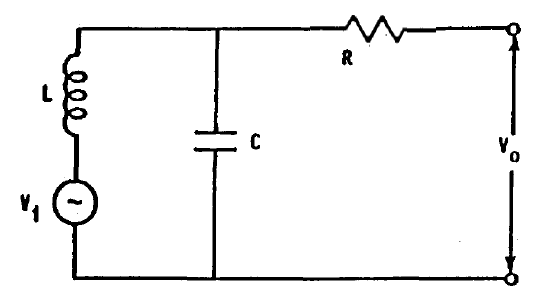
\includegraphics[scale=0.6]{./img/circuitEQ}
	%\fonte{Adaptado de~\citeonline[p.~1358]{kanda1993}}
	\legend{\hspace{-100pt}Fonte: Adaptado de~\citeonline[p.~1358]{kanda1993}}
	\label{fig:circuitEQ}
\end{figure}

Onde, $V_i$ é a tensão induzida (dada pela equação~\ref{FaradayLaw}), $L$ é a auto-indutância, $C$ é a capacitância resultante, e $R$ é a resistência equivalente do circuito (Assumindo que seja independente da frequência) e por fim $V_0$ é a tensão lida sob o circuito. Então a resposta de uma NFP \textit{eletricamente pequena} é dada por:

\begin{eqnarray}
\frac{V_0}{V_i} &=& \frac{-j \frac{1}{\delta }}{\frac{1}{Q} + j \left (\delta - \frac{1}{\delta} \right )} \label{VoVi}
\end{eqnarray}

Onde, $Q = \frac{R}{X_0}$, $X_0 = \omega_0L = \frac{1}{\omega_0C}$, e $\delta = \frac{\omega}{\omega_0}$. Sabendo ainda que $\omega_0 = \frac{1}{\sqrt{L_{i}C_{i}}}$, que é a frequência angular de ressonância, temos que determinar $L$ e $C$, no qual é exposto de forma rigorosa em~\citeonline{kanda1984}, de onde se extrai que:

\begin{eqnarray}
L = \mu b \left \{ln \left ( \frac{8b}{a}  \right ) -2  \right \} \nonumber
\end{eqnarray}

Onde, L é a indutância de uma espira, em que $\mu$ é a permeabilidade do meio, $b$ é o raio da espira, $a$ é o raio do fio que forma a espira. Porém, desde que o raio da espira seja muito maior que o raio do fio, ou seja, $b \gg a$, a indutância $L$ pode ser aproximada por: 

\begin{eqnarray}
L = \mu b ln \left ( \frac{b}{a}  \right )
\end{eqnarray}

~\citeonline{kanda1984} ainda traz que a capacitância da espira pode ser determinada como:

\begin{eqnarray}
C = \frac{2 \epsilon b}{ln \left ( \frac{8b}{a}  \right ) -2 } \nonumber
\end{eqnarray}

Onde, $\epsilon$ é a permissividade do meio que forma a espira. Similarmente ao que ocorre no caso da indutância, se tivermos $ln \frac{b}{a} > 1$, a capacitância da espira pode ser aproximada por:

\begin{eqnarray}
C = \frac{2 \epsilon b}{ln \left ( \frac{b}{a}  \right )}
\end{eqnarray}

Dessa forma, pela equação~\ref{FaradayLaw} que $V_{fem} = V_i  = -j\omega \mu H_nNA$ teremos que a função de transferência de uma espira eletricamente pequena é dada por:

\begin{eqnarray}
FT(f) = \left | \frac{V_0}{H_n} \right | = \omega \mu NA \left | \frac{1}{\frac{1}{Q} + j \left (\delta - \frac{1}{\delta} \right )} \right |
\end{eqnarray}

% Circuito eletromagnetico equivalente
% Equacionamentos
% Tem no funato2006

\subsection{Modelagem como Antena}
% Parametros Fundamentais de Antenas
Uma NFP, além de possuir as características eletromagnéticas expostas anteriormente, também tem propriedades de uma antena do tipo \textit{LOOP} ou circular.

% Loop Antenas
Antenas do tipo \textit{LOOP} podem ser classificadas em duas categorias, eletricamente pequenas e eletricamente grandes. Antenas eletricamente pequenas são aquelas cujo comprimento total (circunferência) é geralmente menor que cerca de um décimo de um comprimento de onda ($C < \lambda / 10$), em contrapartida antenas eletricamente grandes são aqueles cuja circunferência é da ordem do comprimento de onda do espaço livre ($C \sim \lambda $)~\cite[p.~232]{balanis2005}.

\begin{figure}[htb!]
	\centering 
	\caption{Arranjo Geométrico - Análise Antena LOOP}
	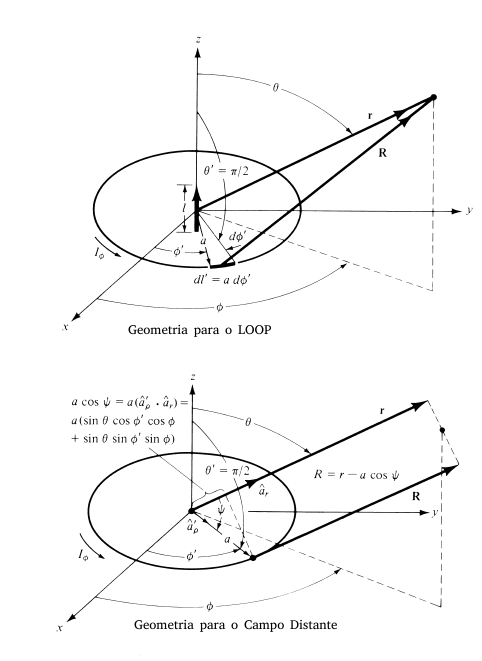
\includegraphics[scale=0.9]{./img/balanis2005_geometria}
	\fonte{Adaptado de~\citeonline[p.~233]{balanis2005}}
	%\legend{\hspace{-100pt}Fonte: Adaptado de~\citeonline[p.~1]{mediano2018}}
	\label{fig:balanis2005_geometria}
\end{figure}

Arranjando geometricamente a antena \textit{LOOP} conforme a figura~\ref{fig:balanis2005_geometria}, ~\citeonline[p.~233]{balanis2005} realizou a análise para obter as componentes do campo magnético e por conseguinte o campo elétrico, sendo que para um \textit{LOOP} pequeno (que pode ser aproximado por um dipolo infinitesimal temos:

\begin{eqnarray}
E_r &=& E_\theta = H_\phi = 0\\
E_\phi &=& -j \frac{k I_m l sin\theta}{4 \pi r} \left [ 1 + \frac{1}{jkr} \right ] e^{-jkr}\\
H_r &=& \frac{I_m l cos\theta}{2\pi \eta r^2} \left [ 1 + \frac{1}{jkr} \right ] e^{-jkr}\\
H_\theta &=& j \frac{k I_m l sin \theta}{4\pi \eta r} \left [ 1 + \frac{1}{jkr} -\frac{1}{(kr)^2} \right ] e^{-jkr}
\end{eqnarray}

Onde, $I_m l = j \omega \mu A I_0$ é o momento de dipolo magnético, sendo $I_0$ a corrente elétrica na espira (nesse caso única).

%A resposta de uma antena, feita de uma espira, é geralmente diretamente proporcional à frequência. Um método para se obter uma resposta plana, em frequência, de uma antena de espira é alterar a impedância da antena com uma resistência de carga no terminal.


\subsection{Grandezas Envolvidas}
Com tudo que vimos até agora, sabemos que os problemas de EMI/EMC estão intimamente relacionados com as correntes no circuito, correntes elétricas operando em altas frequências, sendo estas as responsáveis pelas irradiações nas PCIs, cabos, conectores etc. Devido a este fato, as NFPs, como vimos, são uma ótima ferramenta para identificar essas frequências (sinais). Para isso, comumente se conecta as NFPs em um analisador de espectro para ver as frequências envolvidas no DUT próximo a NFP.~\cite[p.~1]{mediado2018}.

Porém, ainda pode-se surgir a seguinte questão, que grandeza estamos mensurando com a NFP? campo magnético? tensão? ou corrente? Sabe-se que a NFP retorna como informação um valor de tensão elétrica que há de ser aplicado na impedância de entrada do instrumento de medição (Analisador, Osciloscópio, Pré-Amplificado, Filtro, etc.) mas o que exatamente representa este valor de tensão?

\begin{figure}[htb!]
	\centering 
	\caption{Esquema de medidas - Grandezas Envolvidas}
	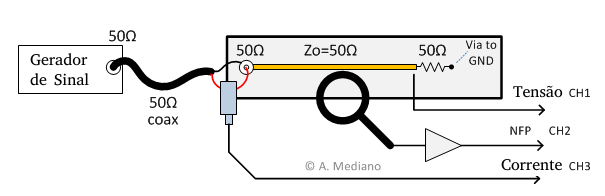
\includegraphics[scale=1]{./img/mediano2018}
	\fonte{Adaptado de~\citeonline[p.~1]{mediado2018}}
	%\legend{\hspace{-100pt}Fonte: Adaptado de~\citeonline[p.~1]{mediano2018}}
	\label{fig:mediano2018}
\end{figure}

Em seu trabalho, ~\citeonline[p.~1]{mediado2018} realizou exatamente esta análise. Na figura~\ref{fig:mediano2018} visualiza-se o esquema de ligação utilizado para investigar quais grandezas estão envolvidas em análises com NFPs, dessa forma ~\citeonline[p.~1]{mediado2018} aplicou sinais senoidais e pulsos quadráticos afim de verificar como se comportam as grandezas envolvidas

\begin{figure}[htb!]
	\centering
 	\caption{Identificação dos Sinais - Grandezas Envolvidas}
	\subfloat[][Sinal Senoidal]{
		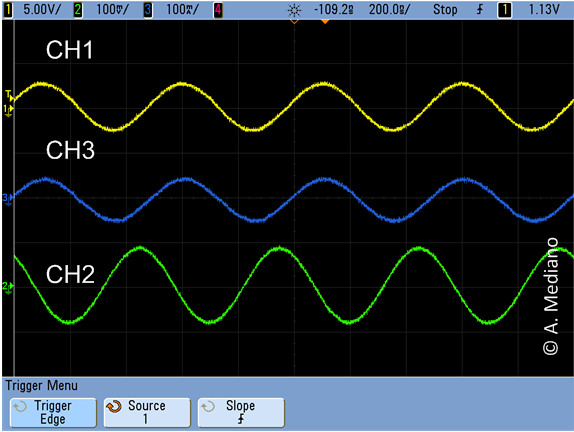
\includegraphics[scale=0.5]{./img/mediado2018_seno}
		\label{fig:mediado2018_seno}}
	\subfloat[][Pulso Quadrático]{
		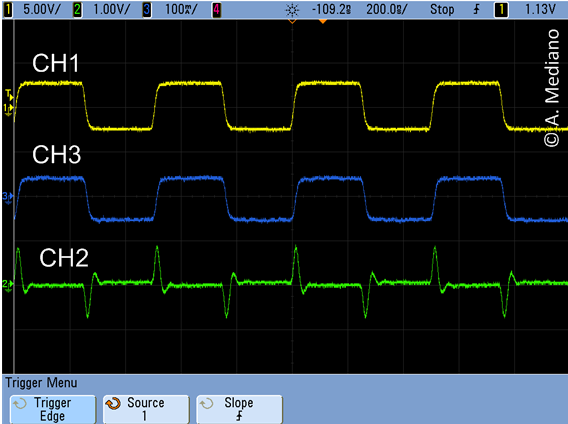
\includegraphics[scale=0.51]{./img/mediano2018_square}
		\label{fig:mediano2018_square}}
    \fonte{Adaptado de~\citeonline[p.~1]{mediado2018}}
\end{figure}

Na figura~\ref{fig:mediado2018_seno}, em seu experimento \citeonline[p.~1]{mediado2018} aplicou no DUT um sinal senoidal de 20MHz, sendo os canais CH1 e CH3 - Tensão e Corrente no DUT, respectivamente, estando estes em fase, devido a termos apenas uma carga puramente resistiva. Porém no canal 2 (CH2), onde esta ligado a NFP, vemos um sinal defasado de $90^{\circ}$. A NFP é sensitiva ao campo magnético, logo a tensão de saída da NFP é proporcional ao campo magnético medido. 

Na figura~\ref{fig:mediano2018_square}, em seu experimento \citeonline[p.~1]{mediado2018} aplicou no DUT um sinal quadrático de 20MHz, notemos agora que o comportamento da NFP é diferente do anterior, haja vista que somente com a variação da corrente $M \frac{\mathrm{d} i}{\mathrm{d} t}$ é que iremos ter variação de fluxo magnético e por conseguinte (Respeitando a lei de Lenz) o aparecimento de uma tensão induzida na espira da NFP.

Diante disto, notemos que, a medida obtida de uma NFP é uma tensão que tem ligação direta com a derivada da corrente no DUT $M \frac{\mathrm{d} i}{\mathrm{d} t}$, sendo $M$ a indutância mútua ou o fator de acoplamento entre a NFP e o DUT.

